%%%%%%%%%%%%%%%%%%%%%%%%%%%%%%%%%%%%%%%%%%%%%%%%%%%%%%%%%%%%%%%%%%%%%%%%%%%%%%%%
%%%%%%%%%% Author: Theo Park
%%%%%%%%%%%%%%%%%%%%%%%%%%%%%%%%%%%%%%%%%%%%%%%%%%%%%%%%%%%%%%%%%%%%%%%%%%%%%%%%
\documentclass{report}
\usepackage[utf8]{inputenc}

\usepackage{algorithm} % Wraps algorithmic env and turns it in to a figure -- I prefer not using it bc of the pagebreak
% algorithmic < algorithmicx < algpseudocode < algpseudocodex -- has indentation guide and LComment that others don't
\usepackage{algpseudocodex}
\algnewcommand{\LineComment}[1]{\State \(\triangleright\) #1} % Line comment env
\usepackage{amsmath} % \text
\usepackage{amssymb} % \therefore
\usepackage{forest} % Treeeeeeeee
\usepackage{hyperref} % hyperlink for toc
\usepackage{import} % better \input \include
\usepackage{multicol}
\usepackage{palatino} % font
\usepackage{tikz} % you know what tikz is

% Pkg used for both header and footer
\usepackage{fancyhdr}
% Header
\topmargin=-0.45in
\evensidemargin=0in
\oddsidemargin=0in
\textwidth=6.5in
\textheight=9.0in
\headsep=0.25in

% Footer
\renewcommand{\footrulewidth}{0.5pt} % Footer line thickness
\rfoot{\small{\textit{By Theo Park, based on Purdue Fall 2022 CS251}}}

% Title page
\title{DSA Mini Textbook}
\author{Theo Park}
\date{}

\begin{document}

\maketitle

\pagestyle{fancy}

% TOC

\tableofcontents

% Preface

\chapter*{Preface}
\addcontentsline{toc}{chapter}{Preface}

% Chapter 1

\chapter{Runtime Analysis}
\import{chapters}{chapter1.tex}

% Chapter 2

\chapter{Intro to Data Structures}

\textit{Data structures} are collections of data values, the relationships among them, and the functions or operations that can be applied to the data. All three characteristics need to be present.

\section{Array}

\textit{Array} is a linear container of items.

\begin{center}
  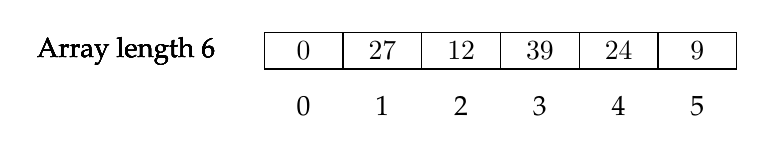
\begin{tikzpicture}
    \foreach \x [ evaluate={\l=int(mod(\x * 69, 42)}; ] in {0,...,5} {
      \node [left] at (-1,1) {Array length 6};
      \node [draw, minimum width=1cm] at (\x, 1) {$\l$};
      \node at (\x, 0.3) {\x};
    } % foreach
  \end{tikzpicture}
\end{center}

\begin{itemize}
  \item Access time: $\Theta (1)$
  \item Inserting $n$ items in the \textit{tail} for array size $n$: $\Theta(1)$ per item, $n \times \Theta(1) \in \Theta(1)$
  \item Inserting $n$ items in the \textit{tail} for array size \textit{unknown}: $\Theta(n)$ per item, $n \times \Theta(n) \in \Theta(n)$
\end{itemize}

Lesson? \textbf{Keep track of the tail!}

\section{Linked List}

\section{Stack}

\section{Queue}

\section{Binary Heap}

\subsection{Building a Heap -- Top-down v.s. Bottom-up}

\section{Tree}

% Chapter 3

\chapter{Sorting Algorithms}
\import{chapters}{chapter3.tex}

% Chapter 4

\chapter{Hash Tables}

\section{Division Method}

\section{Multiplication Method}

\section{Collision}

\subsection{Chaining}

\subsection{Open Addressing}

% Chapter 5

\chapter{Search Tree}

\section{Binary Search Tree and Its Limit}

\section{2-3 Tree}

\section{Red-Black Tree}

\section{Left-Leaning Red-Black Tree}

\subsection{Deletion in LLRBT}

% Chapter 6

\chapter{Graph Traversal}

\section{Adjacency Matrix and List}

\section{DFS}

\section{BFS}

% Chapter 7

\chapter{Directed Graphs}

\section{Strong Connectivity}

\subsection{Brute-force Strong Connectivity Algorithm}

\subsection{Brute-force using Stack}

\subsection{Strongly Connected Components and Kosaraju's Algorithm}

\section{Directed Acyclic Graphs}

\subsection{Topological Sort}

% Chapter 8

\chapter{Weighted Graphs}

\section{Shortest Path}

\subsection{Dijkstra's Algorithm}

\subsection{Bellman-Ford Algorithm}

\section{Articulation Points}

\section{Minimum Spanning Tree}

\subsection{Cycle and Cut Properties}

\subsection{Prim's Algorithm}

\section{Union-Find}

\subsection{Kruskal MST Algorithm}

% Chapter 9

\chapter{Strings}

\section{Brute-force String Pattern Matching}

\section{KMP Algorithm}

\section{Trie}

\section{PATRICIA}

\section{Huffman Coding}

\end{document}
